 \thispagestyle{gocconone}
\pagestyle{gocco}
\everymath{\color{gocco}}
\graphicspath{{../gocco/pic/}}
\blfootnote{$^1${\color[named]{gocco}Trung tâm Quy hoạch và Điều tra tài nguyên -- môi trường biển khu vực phía Nam.}}
\begingroup
\AddToShipoutPicture*{\put(0,616){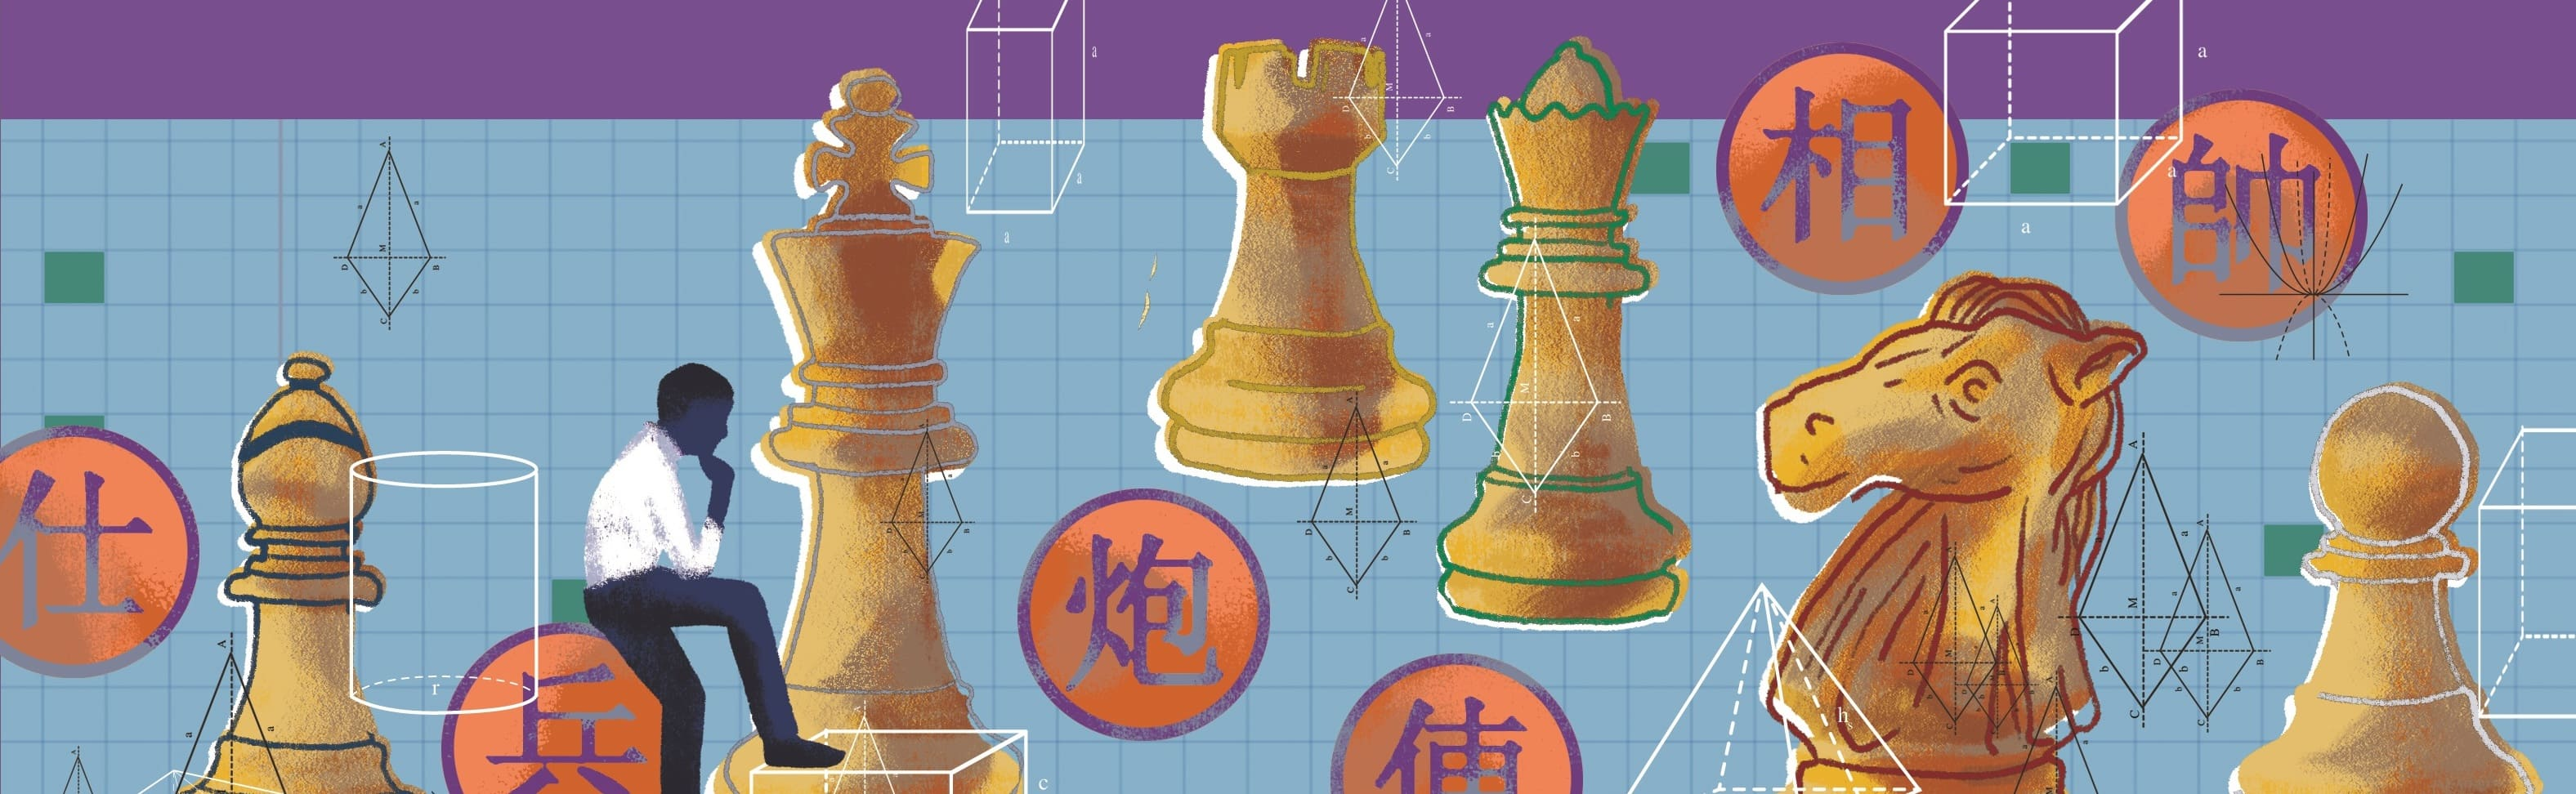
\includegraphics[width=19.3cm]{../bannergocco}}}
\AddToShipoutPicture*{\put(94,520){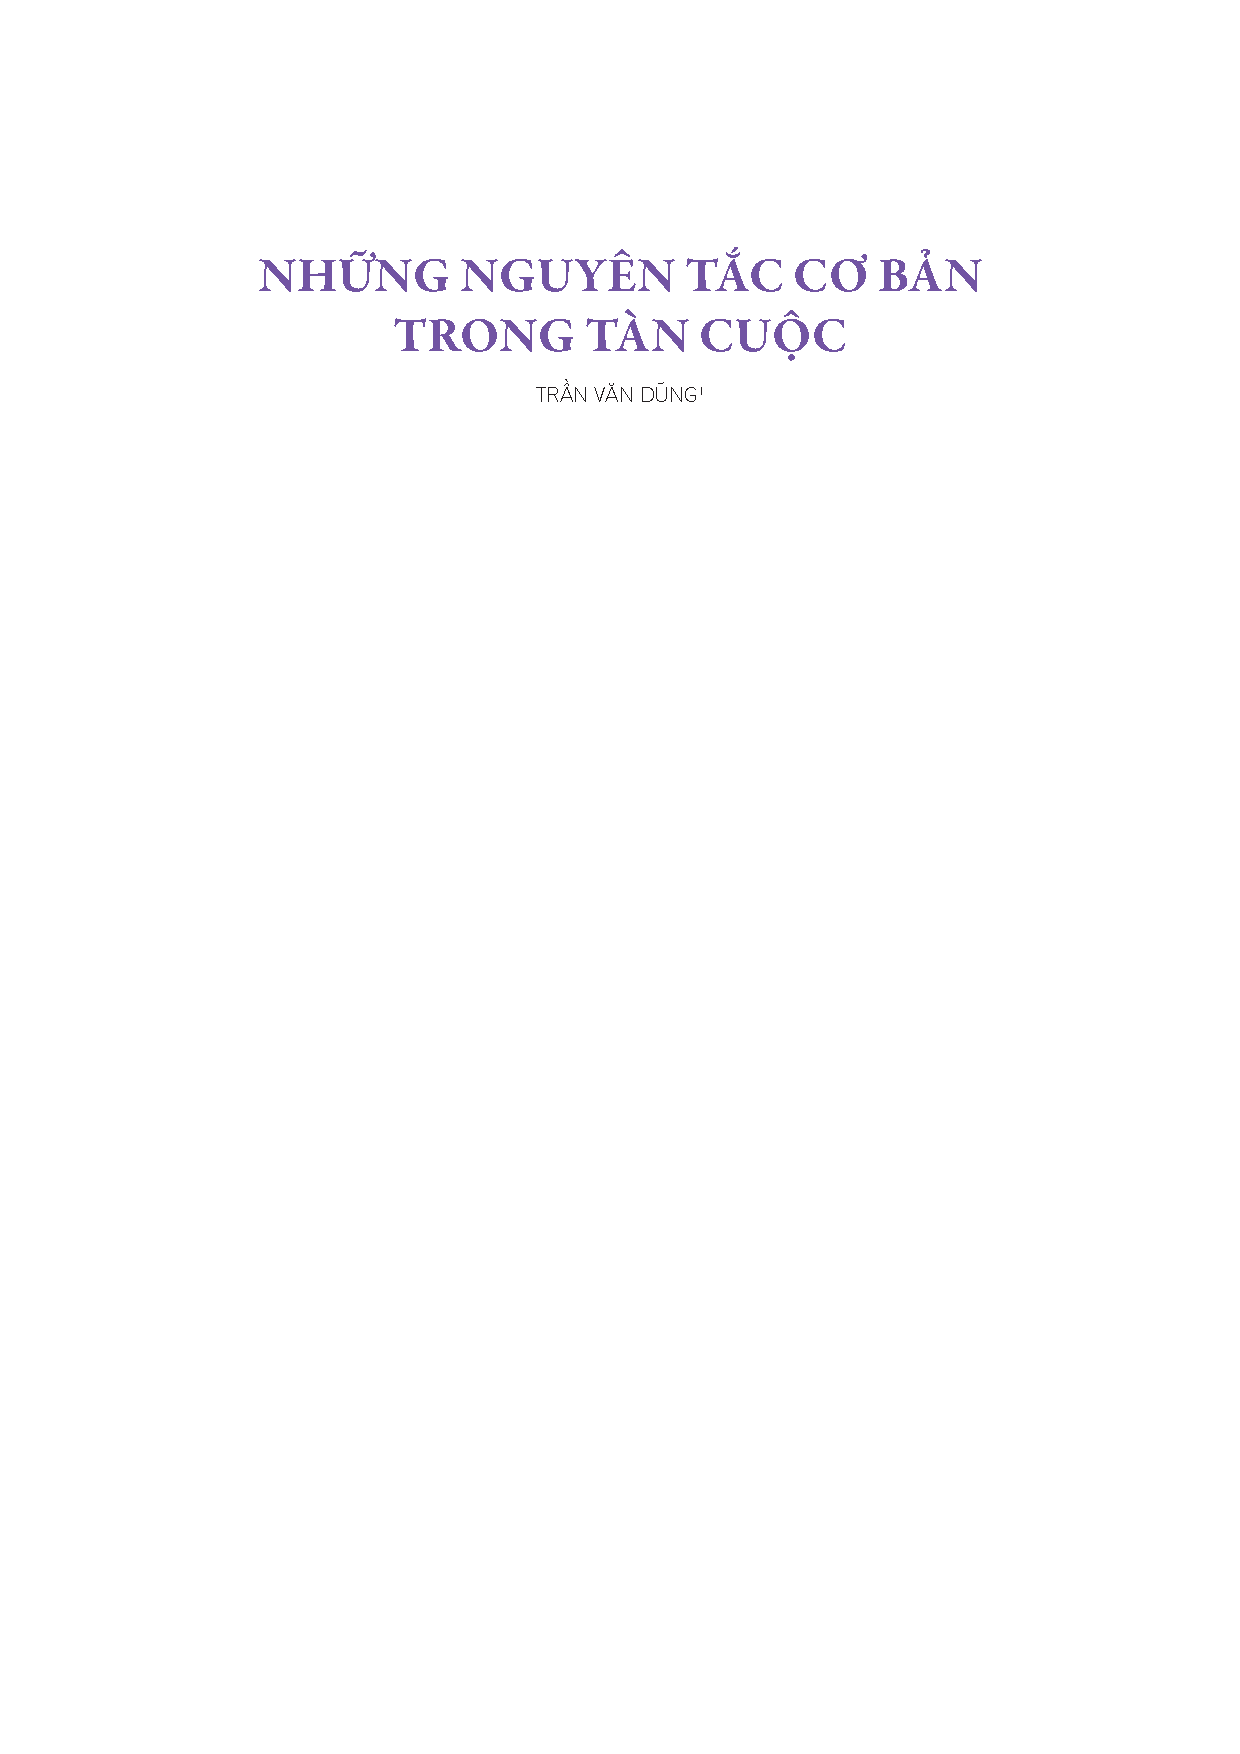
\includegraphics[scale=1]{../tieude.pdf}}} 
\centering
\endgroup

\vspace*{190pt}
\begin{multicols}{2}
	Trong diễn biến của mỗi ván cờ, sau giai đoạn khai cuộc và trung cuộc với hàng loạt những nước cờ điều binh khiển tướng, tranh giành ưu thế cả về lượng và chất, quân số của đôi bên dần bị triệt tiêu, thế trận từ đó cũng trở nên đơn giản, trận đấu sẽ bước vào những nước cờ quyết định cuối cùng. \textit{Tàn cuộc}, đó chính là giai đoạn quyết định thành bại của mỗi ván cờ. Mặc dù vẫn chưa có sự nhất trí rõ rệt giữa những nhà nghiên cứu lý luận Cờ Tướng về việc còn bao nhiêu quân thì bắt đầu bước vào tàn cuộc, nhưng mặc nhiên người ta cũng đồng ý rằng, mỗi bên chỉ còn $1$ đến $2$ quân chủ lực và vài con Chốt, lực lược phòng thủ Sĩ, Tượng thông thường cũng không còn được đầy đủ như ban đầu.
	\vskip 0.1cm
	``\textit{Không có cờ tàn, không thành cao thủ}". Thi đấu ở đẳng cấp càng cao, cờ tàn sẽ càng được các kỳ thủ quan tâm và chú trọng luyện tập nhiều hơn, trình độ cờ tàn cũng là một tiêu chuẩn cần thiết để đánh giá trình độ của một kỳ thủ. Trải qua bề dày lịch sử phát triển lâu đời của Cờ Tướng, hàng trăm, hàng nghìn thế cờ tàn đã được các nhà nghiên cứu đem ra phân tích, mổ xẻ một cách tỉ mỉ, từ đó đã rút ra những kết luận về hướng tấn công, phòng thủ hiệu quả cho những hình cờ tàn cụ thể. Tuy nhiên, trước khi nghiên cứu cụ thể về các thế cờ tàn nêu trên, người chơi cần nắm được một số nguyên lý cơ bản như sau:
	\vskip 0.1cm
	$1.$ \textit{Các quân cần liên kết, phối hợp liên hoàn}
	\vskip 0.1cm
	Số lượng quân trong tàn cuộc còn lại rất ít, giá trị của mỗi quân đều tăng lên, nhất là khi chúng chiếm được những vị trí quan trọng. Việc liên kết,  phối hợp liên hoàn, giúp các quân càng tăng thêm sức mạnh, thuận lợi cho cả tấn công và phòng thủ. 
	\vskip 0.1cm
	$2.$ \textit{Bảo vệ tối đa lực lượng, đổi quân đúng thời điểm}
	\vskip 0.1cm
	Nếu đã chiếm ưu thế trong cờ tàn, không nên đổi quân khi chưa chuyển được về thế thắng điển hình, lại càng không được phép hy sinh vô tội vạ, bất kể đó là Chốt Sĩ hay Tượng, mỗi quân đều có thể là nhân tố quan trọng góp phần vào thắng lợi của cuộc cờ.
	\vskip 0.1cm
	$3.$ \textit{Linh hoạt giữa tấn công và phòng thủ}
	\vskip 0.1cm
	Nguyên tắc này không hề mâu thuẫn vơi nhau, mà người chơi cần phải ứng biến kịp thời cho những tình huống cụ thể. Đừng quá mải mê tấn công mà quên bảo vệ Tướng bên mình, cũng nhưng đừng co cụm phòng thủ mà bỏ quên những cơ hội chiến thắng.
	\vskip 0.1cm
	$4.$ \textit{Chú ý chiếm các trục lộ quan trọng}
	\vskip 0.1cm
	Khi còn ít quân, các trục lộ $4$, $5$, $6$ càng trở nên quan trọng vì nó đi ngang qua Cửu Cung, là nơi hoạt động của Tướng. Việc khống chế và chiếm lĩnh các trục lộ này có ý nghĩa quyết định đến việc giành thắng lợi sau cùng.
	\vskip 0.1cm
	$5.$ \textit{Vận dụng Tướng, Sỹ và Tượng k hi tấn công}
	\vskip 0.1cm
	Nếu có đầy đủ Sỹ Tượng sẽ dễ dàng phòng thủ, bảo vệ sự an toàn của Tướng. Tuy nhiên, những quân này vẫn có thể hỗ trợ làm ngòi cho Pháo, mở mặt để truy kích Tướng đối phương khi cần thiết, hãy biết cách khai thác triệt để sức mạnh của chúng.
	\vskip 0.1cm
	$6.$ \textit{Tận dụng sức mạnh của Chốt}
	\vskip 0.1cm
	Những quân Chốt trong cờ tàn cực kỳ quan trọng. Một khi đã vượt sông, sức mạnh của chúng tăng lên gấp bội, có thể gây áp lực không hề nhỏ lên trận địa đối phương. Hãy bảo vệ và khéo léo vận dụng Chốt, bạn sẽ thấy được hiệu quả bất ngờ.
	\vskip 0.1cm
	Dưới đây là một vài ví dụ điển hình về việc áp dụng các nguyên tắc trong cờ tàn để bạn đọc của Pi tham khảo:
	\begin{figure}[H]
		\vspace*{-5pt}
		\centering
		\captionsetup{labelformat= empty, justification=centering}
		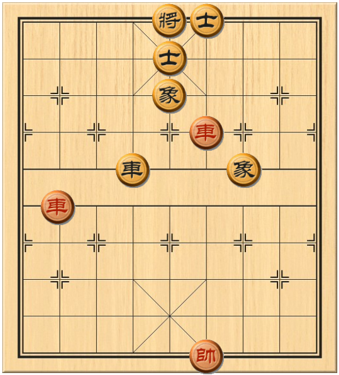
\includegraphics[width= 0.38\textwidth]{1}
		\caption{\small\textit{\color{gocco}Hình $1$.}}
		\vspace*{-10pt}
	\end{figure}
	$1$. Hình $1$, bên đỏ còn song Xe, bên Đen còn $1$ Xe nhưng đầy đủ Sỹ tượng. Trong tình huống thông thường, Đen chỉ cần đổi Xe là đưa về thế cờ hòa cơ bản. Nhưng với việc đỏ đã khống chế trục lộ $4$, cộng với việc vị trí của Tượng Đen không đẹp, Đỏ không cho Đen có một cơ hội nào để thực hiện ý đồ đổi quân. Đỏ ra đòn như sau:
	\vskip 0.1cm
	$\pmb{1)}$	X$8.5$ X$4/4$\quad $\pmb{2)}$ X$8/2$  T$5/7$\quad $\pmb{3)}$ X$8-3$ Tt$/9$($*$)\quad $\pmb{4)}$ X$4.2$ X$4.3$ \quad$\pmb{5)}$ X$4-2$ X$4-6$\quad $\pmb{6)}$ Tg$4-5$ X$6-5$\quad $\pmb{7)}$ Tg$5-4$ S$5/4$\quad $\pmb{8)}$ X$3-4$ S$4.5$\quad $\pmb{9)}$ X$4-1$($**$) ($1-0$)
	\vskip 0.1cm 
	\textit{($*$): Với việc $1$ Xe và Tướng đã chiếm trục lộ $4$ khiến Đen không thể đảo Sĩ, Đỏ sử dụng Xe còn lại liên tục có những đòn tấn công thị uy sức mạnh, trước ép Xe Đen lui về tuyến đáy phòng thủ, sau lại đẩy đôi Tượng qua vị trí xấu hơn để dễ dàng uy hiếp.
	\vskip 0.1cm
	($**$): Tiếp đó, Đỏ lại có những nước điều Xe nhằm chia cắt và bắt sống Tượng. Đen đã cố gắng dùng Xe để chiếm trục lộ $5$ nhưng có vẻ như mọi thứ đã quá muộn. Đỏ bắt chết $1$ Tượng, dễ dàng giành lấy chiến thắng.}
	\begin{figure}[H]
		\vspace*{-5pt}
		\centering
		\captionsetup{labelformat= empty, justification=centering}
		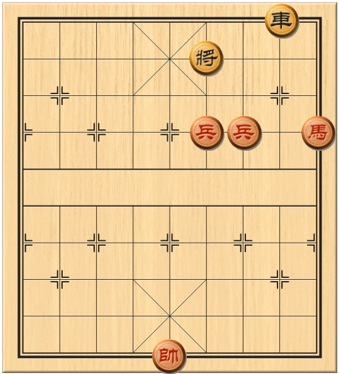
\includegraphics[width= 0.38\textwidth]{3}
		\caption{\small\textit{\color{gocco}Hình $2$.}}
		\vspace*{-10pt}
	\end{figure}
	$2.$ Hình $2$, có vẻ như Đen đang có lợi thế lớn vì còn Xe, chỉ cần chiếm trung lộ là Đỏ lập tức rơi vào tình thế nguy hiểm. Nhưng Đỏ lại được quyền đi trước, lập tức có những nước điều Mã Chốt tấn công liên hoàn rất hay như sau:
	\vskip 0.1cm
	$\pmb{1)}$ C$4.1$($*$) Tg$6.1$\quad $\pmb{2)}$ C$3.1$ Tg$6/1$\quad $\pmb{3)}$ C$3.1$ Tg$6/1$($**$)\quad $\pmb{4)}$ M$1.2$ X$8-9$\quad $\pmb{5)}$ M$2/3$($***$ ($1-0$)
	\vskip 0.1cm
	\textit{($*$): Nhận thức được sự nguy hiểm của Xe Đen, Đỏ mạnh dạn phế Chốt, giành lấy tiên thủ.
	\vskip 0.1cm 
	($**$): Đỏ tiếp tục những nước tấn công liên tiếp, buộc Tướng phải lui về tuyến đáy để né tránh, và điều này cũng vô tình ngăn cản khiến cho Xe Đen chưa thể bình vào trung lộ để tấn công ngược lại. ``Nhất tiễn hạ song điêu", Đỏ đã đạt được mục đích ban đầu của mình.
	\vskip 0.1cm
	($***$): Nhảy liên tiếp $2$ nước Mã đầy khéo léo, Đỏ đe dọa nước tiếp theo dùng Chốt bắt chết Tướng đối phương. Lúc này Xe Đen đã có thể di chuyển nhưng mọi thứ đã quá muộn, Đỏ giành thắng lợi.}
	\begin{figure}[H]
		\vspace*{-5pt}
		\centering
		\captionsetup{labelformat= empty, justification=centering}
		
\includegraphics[width= 0.38\textwidth]{2}
		\caption{\small\textit{\color{gocco}Hình $3$.}}
		\vspace*{-10pt}
	\end{figure}
	$3$. Hình $3$, đôi bên đang có quân lực khá đồng đều, đỏ chỉ hơn $2$ Tượng. Nếu xảy ra tình huống đổi quân, ván cờ sẽ nhanh chóng có kết quả hòa. Tuy nhiên Đỏ rất biết vận dụng tối đa sức mạnh các quân còn trên bàn cờ để giành chiến thắng như sau: 
	\vskip 0.1cm
	$\pmb{1)}$ S$5.6$ X$4.1$($*$)\quad $\pmb{2)}$ X$6/1$ X$4.2$\quad $\pmb{3)}$ Tg$5.1$ X$4-9$\quad $\pmb{4)}$ X$4-6$ Tg$4-5$($**$)\quad $\pmb{5)}$ Tg$5-6$ X$9/3$\quad  $\pmb{6)}$ X$6.3$ M$8/7$\quad $\pmb{7)}$P$3-5$ M$7/5$\quad $\pmb{8)}$ X$6-5$ Tg$5-6$\quad $\pmb{9)}$ P$5-4$($***$) ($1-0$)
	\vskip 0.1cm
	\textit{($*$): Đỏ có nước treo Sĩ đầy tinh tế, ép Xe Đen phải ăn xuống. Từ đó Đỏ lùi Xe chiếm lấy đường ngang dãy Chốt, qua đó dọa đi X$4-2$ bắt chết Mã đối phương.
	\vskip 0.1cm
	($**$): Để tránh mất quân, Đen buộc phải dùng nước chiếu để dạt xe ra biên giữ Mã. Không thể bỏ lỡ thời cơ, Đỏ bình xe chiếm lộ $6$ ngay lập tức.
	\vskip 0.1cm
	($***$): Liên tiếp là những nước tận dụng để Sĩ Tượng hỗ trợ Pháo uy hiếp Tướng của Đỏ, Xe -- Mã Đen không thể phòng thủ kịp thời, Đen chấp nhận thua cuộc.}
	\vskip 0.1cm
	\textit{Chú thích}: C: Chốt, X: Xe, M: Mã, P: Pháo, Tg: Tướng, S: Sĩ, T: Tượng. t: trước
	\vskip 0.1cm
	\textbf{\color{gocco}Câu đố kỳ này:} Đỏ được quyền đi trước, sẽ chơi như thế nào để giành thắng lợi trong các hình cờ tàn dưới đây:
	\begin{figure}[H]
		\vspace*{-5pt}
		\centering
		\captionsetup{labelformat= empty, justification=centering}
		
\includegraphics[width= 0.38\textwidth]{4}
		\caption{\small\textit{\color{gocco}Hình $4$.}}
		\vspace*{-10pt}
	\end{figure}
%	\textit{Đáp án tham khảo:}
%	\vskip 0.1cm
%	$\pmb{1)}$	M$6.7$ Tg$4.1$\quad $\pmb{2)}$ C$5-6$ M$5.3$\quad $\pmb{3)}$ M$7/5$ Tg$4/1$\quad $\pmb{4)}$ C$6.1$ Tg$4-5$\quad $\pmb{5)}$ Tg$5-4$ T$7.9$\quad $\pmb{6)}$ C$6.1$ M$3.4$\quad $\pmb{7)}$ M$5.7$ ($1-0$)
%	\vskip 0.1cm
	\begin{figure}[H]
		\vspace*{-5pt}
		\centering
		\captionsetup{labelformat= empty, justification=centering}
		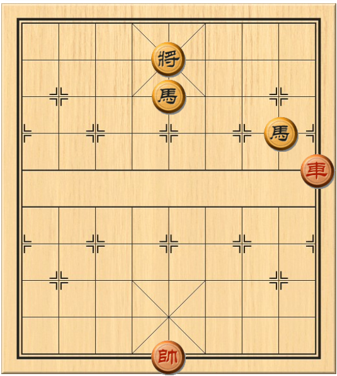
\includegraphics[width= 0.38\textwidth]{5}
		\caption{\small\textit{\color{gocco}Hình $5$.}}
		\vspace*{-10pt}
	\end{figure}
%	\textit{Đáp án tham khảo:}
%	\vskip 0.1cm
%	$\pmb{1)}$ X$1-5$ M$8/7$\quad $\pmb{2)}$ X$5.1$ Tg$5/1$\quad $\pmb{3)}$ X$5-3$ Tg$5-4$\quad $\pmb{4)}$ X$3-6$ Tg$4-5$\quad $\pmb{5)}$ X$6.1$ Tg$5.1$\quad $\pmb{6)}$ X$6-8$ Tg$5-4$\quad $\pmb{7)}$ X$8.1$ Tg$4/1$\quad $\pmb{8)}$ X$8-5$ ($1-0$)
\end{multicols}




